
\chapter{Application to specific families}

In \cite{Vajda2009} authors present formulas for computing and evaluating R\'{e}nyi pseudodistance estimator in normal family. Our goal was to study these estimators in other families. In the next chapter we present our results together with some examples.

\section{Laplaceova distribuce}


We use min R\'{e}nyi estimators for estimating parameter $\theta = (\mu,\lambda)$ in the Laplace family, where the probability density is 
\begin{equation}
	p_\theta = \frac{1}{2\lambda} e^{-\frac{|x-\mu|}{\lambda}}
\end{equation}
and therefore the estimator according to \eqref{Renyi-estimator_formula} is 
\begin{equation}
	\theta_{\alpha,n} = \arg \max_{\theta \in \Theta} \left[ (2\lambda)^{-\frac{\alpha}{1+\alpha}} \frac{1}{n} \sum_{i=1}^n \exp \left[-\alpha\frac{|x_i-\mu|}{\lambda} \right] \right].
\end{equation}
% tabulka a obrazek eref %%%%%%

\begin{table}[htb] \footnotesize
\begin{center}
\begin{tabular}{ccc}
	\begin{tabular}{|c|ccc|} 
	\hline 
	$\alpha\backslash n$ &&  $500$ & \\ 
	\hline 
	& $m(\mu)$ & $s(\mu)$ & $eref(\mu)$ \\ 
	& $m(\lambda)$ & $s(\lambda)$ & $eref(\lambda)$ \\ 
	\hline 
	$0.0$ & $ -0.005 $ & $ 0.071 $ & $ 1.000 $\\ 
	 & $ 4.593 $ & $ 3.617 $ & $ 1.000 $\\ 
	\hline 
	$0.05$ & $ -0.000 $ & $ 0.071 $ & $ 1.018 $\\ 
	 & $ 4.168 $ & $ 3.192 $ & $ 1.284 $\\ 
	\hline 
	$0.1$ & $ 0.003 $ & $ 0.066 $ & $ 1.163 $\\ 
	 & $ 3.719 $ & $ 2.741 $ & $ 1.742 $\\ 
	\hline 
	$0.2$ & $ -0.002 $ & $ 0.068 $ & $ 1.098 $\\ 
	 & $ 2.888 $ & $ 1.914 $ & $ 3.570 $\\ 
	\hline 
	$0.3$ & $ -0.004 $ & $ 0.068 $ & $ 1.108 $\\ 
	 & $ 2.215 $ & $ 1.241 $ & $ 8.490 $\\ 
	\hline 
	$0.5$ & $ 0.001 $ & $ 0.069 $ & $ 1.056 $\\ 
	 & $ 1.546 $ & $ 0.568 $ & $ 40.516 $\\ 
	\hline 
	$1.0$ & $ 0.003 $ & $ 0.074 $ & $ 0.927 $\\ 
	 & $ 1.221 $ & $ 0.256 $ & $ 199.663 $\\ 
	\hline 
	\end{tabular}
&&
	\begin{tabular}{c}
		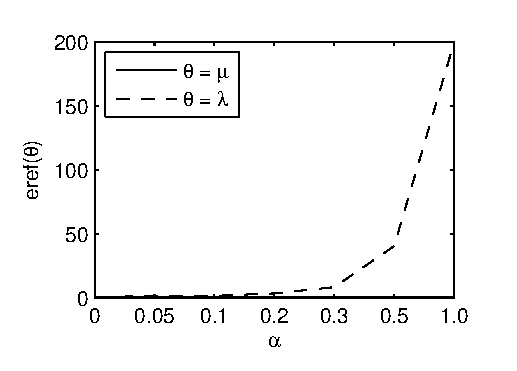
\epsfig{file=Laplace-e04-eref.eps, height=2in} 
	\end{tabular}
\\
\end{tabular}
\end{center}
\caption{R\'{e}nyi: $p_\theta = \mathrm{L}(0,1)$, data: $(1-\varepsilon)\mathrm{L}(0,1) + \varepsilon \mathrm{L}(0,10)$, $\varepsilon =  0.4$} 
\label{tabJK:laplace-eref}
\end{table}
For creation of Table \ref{tabJK:laplace-eref} we generated contaminated data (number of observations $n = 500$) as a mixture of two Laplace distributions $(1-\varepsilon)\mathrm{L}(0,1) + \varepsilon \mathrm{L}(0,10)$ with $\varepsilon =  0.4$. 
Then we used R\'{e}nyi estimators and estimated the parameters $\mu, \; \lambda$ and repeated this process $m = 1000$ times. Numbers in the table are mean value and variance of the estimated parameters. In the last column, there is relative efficiency given by
\begin{equation}
eref(p) = \sqrt{\dfrac{\frac{1}{m}\sum_{k=1}^m (\hat{p}_{\mathrm{MLE} ,k} - p_{\mathrm{real}})^2}{\frac{1}{m}\sum_{k=1}^m (\hat{p}_{\alpha,k} - p_{\mathrm{real}})^2}},
\end{equation}
where $ \hat{p}_{\mathrm{MLE},k}$ is MLE estimator, $p_{\mathrm{real}}$ is the real parameter of the contaminated distribution and $\hat{p}_{\alpha,k}$ is minimal R\'{e}nyi estimator. As we can see, the efficiency raises with increasing $\alpha$. This depends on the level of contamination, estimators with higher $\alpha$ are more robust against outliers, so with increasing level of contamination with more dispersed observations the relative efficiency will raise, because of the robustness against outliers.

%%%%%%%%%%%%%%%%%%%%%%%%%%%%%%%%% laplace - IF %%%%%%%%%%%%%%%%%%%%%%%%%%%%%%%%%%%%%%%
If we compute the influence functions according to \eqref{IF}, where we put $\theta = \mu$ (estimated parameter), $ \lambda := 1$ (known parameter) respectively $\theta = \lambda$, $ \mu := 0$, we get 
\begin{equation}
	\mathrm{IF}(x;T_{\mathfrak{R}_\alpha},\mu) = (1+\alpha )^{\frac{3}{2}} (x-\mu )  e^{-\frac{\alpha}{2} (x-\mu )^2}, % IF(x,mu)
	\label{JK-IF-laplace-mu}
\end{equation}
respectively
\begin{equation}
	\mathrm{IF}(x;T_{\mathfrak{R}_\alpha},\lambda) = (1 + \alpha)^2 \left(-\lambda + (1 + \alpha)|x|\right)  e^{-\frac{\alpha|x|}{\lambda}}	. 
% IF(x,sigma)
	\label{JK-IF-laplace-lambda}
\end{equation}
\begin{figure}[htb]
\begin{center}
\begin{tabular}{c c c}
	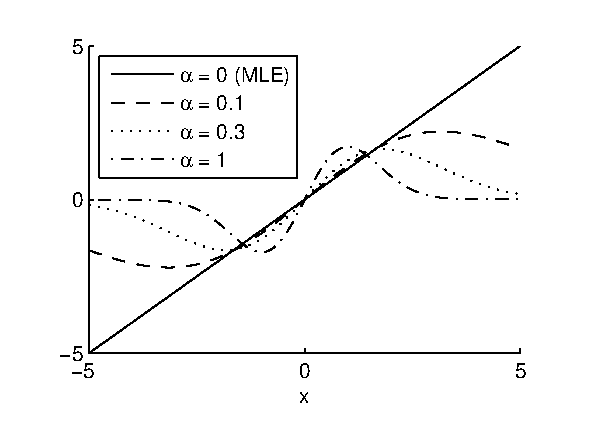
\epsfig{file=Laplace-IF-mu.eps, height=2in} 
	&&
	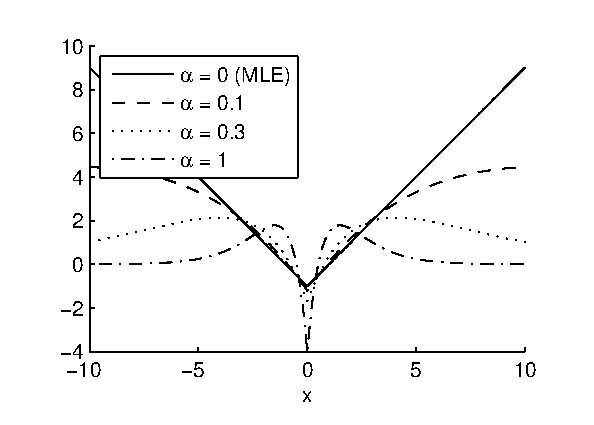
\epsfig{file=Laplace-IF-lambda.eps, height=2in} 
	\\
	$\mathrm{IF}(x;T_{\mathfrak{R}_\alpha},\mu = 0) $, $\lambda = 1$ is known
	&&
	$\mathrm{IF}(x;T_{\mathfrak{R}_\alpha},\lambda = 1)$, $\mu = 0$ is known
	\\
\end{tabular}
\caption{Influence functions of R\'{e}nyi estimator for Laplace distribution}
\end{center}
\label{figJK:laplace-if}
\end{figure}
We can see from \eqref{JK-IF-laplace-mu}, \eqref{JK-IF-laplace-lambda}, that our estimators are robust for $\alpha > 0$ in the sense that their influence functions are bounded. Also with higher $\alpha$ they are robust against outliers, because $\lim_{x\rightarrow \pm\infty}\mathrm{IF}(x;T_{\mathfrak{R}_\alpha},\cdot) = 0 $ and the convergence is faster with increasing $\alpha$ because of the $e^{-\alpha x}$ which appears in both functions.

